\begin{figure}[h]
    \begin{subfigure}{.5\textwidth}
        \centering
        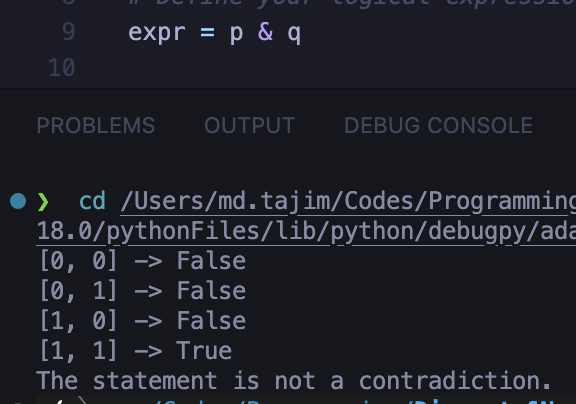
\includegraphics[width=.8\linewidth]{images/output/7pANDq.png}
        \caption*{}
        \label{fig:sfig1}
    \end{subfigure}
    \begin{subfigure}{.5\textwidth}
        \centering
        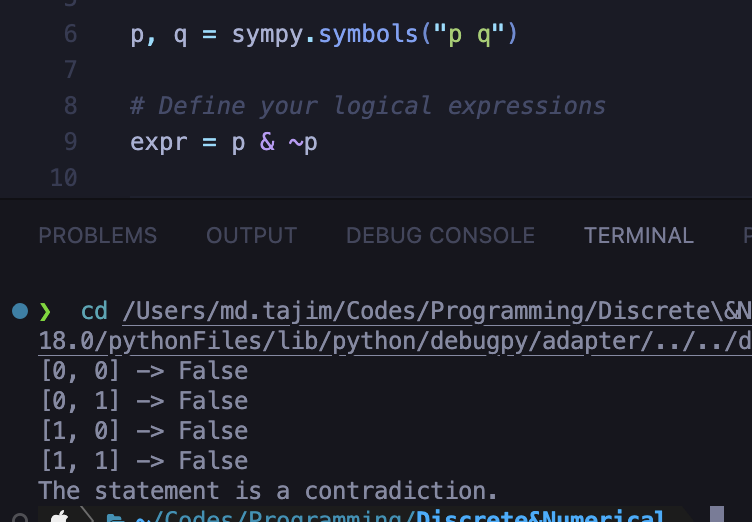
\includegraphics[width=.8\linewidth]{images/output/8pAND~p.png}
        \caption*{}
        \label{fig:sfig2}
    \end{subfigure}
    \begin{subfigure}{1\textwidth}
        \centering
        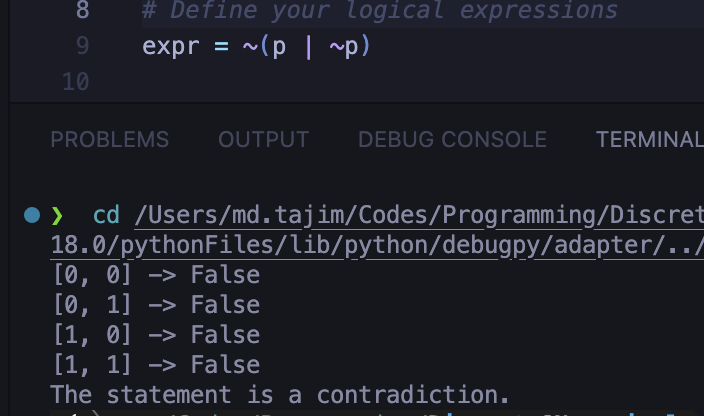
\includegraphics[width=.5\linewidth]{images/output/9~pOR~P.png}
        \caption*{}
        \label{fig:sfig3}
    \end{subfigure}
    \caption{Outputs for Contradiction}
    \label{fig:fig}
\end{figure}

\begin{figure}[h]
    \begin{subfigure}{1\textwidth}
        \centering
        
\includegraphics[width=.8\linewidth]{images/output/4contrap.png}
        \caption*{}
        \label{fig:sfig1}
    \end{subfigure}
    \begin{subfigure}{1\textwidth}
        \centering
        
\includegraphics[width=.8\linewidth]{images/output/5contrap.png}
        \caption*{}
        \label{fig:sfig2}
    \end{subfigure}
    \begin{subfigure}{1\textwidth}
        \centering
        
\includegraphics[width=.8\linewidth]{images/output/6contrap.png}
        \caption*{}
        \label{fig:sfig3}
    \end{subfigure}
    \caption{Outputs for Contraposition}
    \label{fig:fig}
\end{figure}

\begin{figure}[h]
    \begin{subfigure}{.5\textwidth}
        \centering
        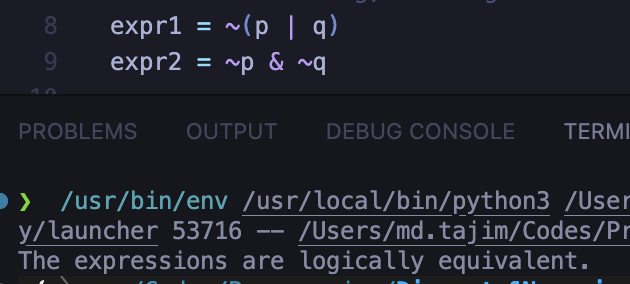
\includegraphics[width=.8\linewidth]{images/output/1demorganOR.png}
        \caption*{}
        \label{fig:sfig1}
    \end{subfigure}
    \begin{subfigure}{.5\textwidth}
        \centering
        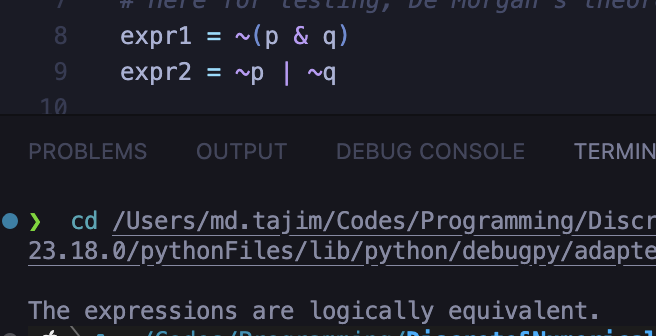
\includegraphics[width=.8\linewidth]{images/output/2demorganAND.png}
        \caption*{}
        \label{fig:sfig2}
    \end{subfigure}
    \begin{subfigure}{1\textwidth}
        \centering
        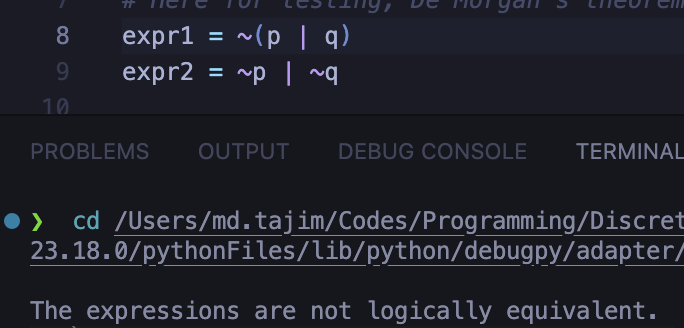
\includegraphics[width=.5\linewidth]{images/output/3random.png}
        \caption*{}
        \label{fig:sfig3}
    \end{subfigure}
    \caption{Outputs for Logical Equivalence}
    \label{fig:fig}
\end{figure}